% IFY TEST
\documentclass[12pt,a4paper,final]{report}
\usepackage[utf8]{inputenc}
\usepackage[T1]{fontenc}
\usepackage{lmodern}
\usepackage[slovak]{babel}
\usepackage{helvet}
\usepackage{amsmath}
\usepackage[dvipdf]{graphicx}
\usepackage{titlesec}
\usepackage{multicol}

\usepackage[unicode,pdfpagelabels,colorlinks,plainpages=false,urlcolor=blue,linkcolor=red]{hyperref}
\usepackage[top=2cm, left=2.5cm, text={16cm, 26cm}, ignorefoot]{geometry}

\titleformat{\section}{\large\bfseries\sffamily\MakeUppercase}{\thesection}{1em}{}
\titleformat{\subsection}{\normalsize\bfseries\sffamily\MakeUppercase}{\thesection}{1em}{}

\setlength{\parindent}{2em}
\setlength{\parskip}{1em}

\begin{document}

\begin{figure}[h!]
	\centering
	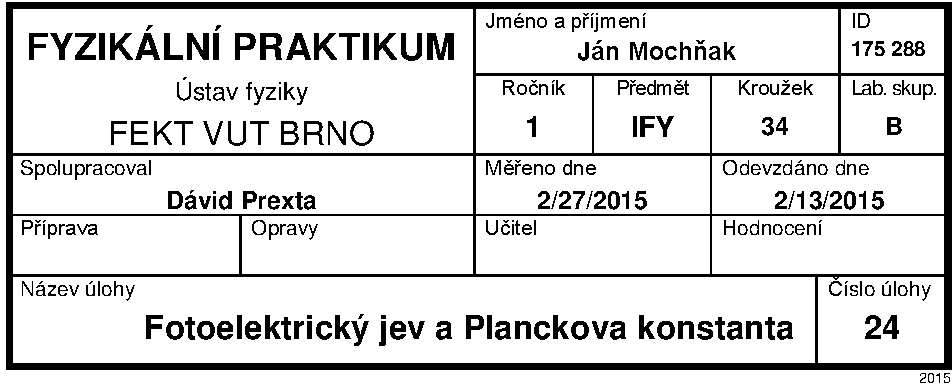
\includegraphics[scale=1,clip=true]{IFY24-crop.pdf}
\end{figure}

\section*{Úkol měření}
Stanovte Planckovu konštantu z merania vonkajšieho fotoelektrického javu a určte výstupnú prácu použitej fotónky.

\section*{TEORETICKÁ PRÍPRAVA}
Pri vysvetľovaní javou spojených so svetlom bolo nutné siahnuť ku dvom rôznym spôsobom popisov. Spôsoby sú navzájom veľmi odlišné, že nutnosť ich koexistencie pri vysvetľovaní bola neuveriteľná. Difrakcia či interferencia spoľahlivo vysvetlí vlnovú teóriu svetla, ale úplne zlyhá pri pokuse objasniť fotoelektrický jav. Pri nej bola úspešná teória kvantová, ktorá naopak nedokáže predpovedať existenciu javov difrakcie. Pri určení udalostí vykazuje svetlo buď vlnovú alebo časticovú povahu, nikdy však oboje zároveň.

Svetlo ako vlnenie charakterizujeme frekvenciou $f$ alebo vlnovou dĺžkou $\lambda$. 

\begin{equation} \label{eq:vlnenie}
	\lambda = \frac{c}{f}
\end{equation} $c$ je rýchlosť šírenia svetla vo vákuu ($2.998\cdot10^8\text{ m.s}^{-1}$).

Pre častice je opäť charakteristiká energia $E$ a hybnosť $p$. Tieto dva prístupy sú navzájom prepojené vzťahmi:
\begin{equation} \label{eq:energia}
	E=hf
\end{equation}
\begin{equation} \label{eq:hybnost}
	p=h\frac{f}{c}=h\frac{1}{\lambda}
\end{equation}Spoločným parametrom je Planckova konštanta $h$. Jedná sa o univerálnu fyzikálnu konštantu s hodnotou $h=6.626\cdot10^{-34}\text{ J.s}$. Často môže byť táto konštanta tiež vyjadrená vo tvare $\hbar=\cfrac{h}{2\pi}$, ktorý sa potom objavuje spoločne s kruhovou frekvenciou $\omega$ a upravuje vzťah energie~\eqref{eq:energia}:
\begin{equation} \label{eq:energia2}
	E=\hbar\omega
\end{equation}
Číselnú hodnotu Planckovej konštanty je možné uvádzať v [eV$\cdot$s] namiesto [J$\cdot$s]. Prevodný vzťah je 1 eV $= 1.602\cdot10^{-19}$ J a hodnota Planckovej konštanty je potom $h=4.136\cdot 10^{-15}$ eV$\cdot$s. Často sa používa v atómovej fyzike.

\subsection*{Stanovenie Planckovej konštanty}
Pre stanovenie Planckovej konštanty využijeme fotoelektrický jav -- je jedným z dôkazov kvantovej povahy elektromagnetického žiarenia. Nastávaa pri vzájomnom pôsobení elektromagnetického žiarenia a látky. Energia žiarenia je pri tom predávana elektronóm v látke.

Máme dva typy fotoelektrického javu vnútorný a vonkajší. Vnútorny jav je pre náš prípad nevyhovujúci. Je to hlavne z dôvodu, že je typický pre polovodiče a dielektriká.

Vonkajší jav vysvetlil A. Einstein v roku 1905. Elektromagnetické žiarenie frekvencie $f$ je pohlcované v kvantách, fotónov, ktorých energia $E$ je frekvencii $f$ úmerná. Tento vzťah je popísaný rovnicou~\eqref{eq:energia}, kde konštantou úmernosti je hľadaná Planckova konštanta. Fotoelektrón, ktorý absorboval fotón môže opustiť povrch ožiarenej látky iba ak pohltená energia je väčšia, ako energia potrebná k tomu, aby sa dostal z látky von. Táto eneriga sa označuje symbolom $W$ - názov výstupnej práce. Po opustení povrchu látky zostáva fotoelektrónu kinetická energia $E_K$:
\begin{equation} \label{eq:kinetickaEnergia}
	E_K=hf-W
\end{equation}.

Keď sa vo vákuu priblížime k fotoelektróde (osvetlenej látke) ďalšiou elektródou (zbernou), budú na ňu dopadať fotoelektróny. Ak spojíme obidve elektródy vonkajším obvodom začne pretekať prúd, pričom súčiastka, ktorá pracuje na popísanom princípe sa nazýva \textit{vákuová fotónka}.

Vložíme medzi obidve elektródy fotónky napätie $U$ tak, že fotoelektróda bude kladná voči zbernej elektróde, budú fotoelektróny svojej ceste medzi fotoelektódou a zbernou elektródou brzdené. So vzrastajúcim napätím s prúd obvodom zmenšuje. Pri určitom $U=U_b$ prúd obvodom ustane. Práca $e\cdot U_b$, ktorá je potrebná v brzdiacom elektrickom poli vykonať pri priechode medzi obomi elektródami, dosiahla práve hodnoty kinetickej energie $E_K$ ktorú má fotoelektrón k dispozícii. Preto platí:
\begin{equation} \label{eq:eUb}
	eU_b=E_K=hf-W
\end{equation}
a pre brzdné napätie:
\begin{equation} \label{eq:Ub}
	U_b=\cfrac{h}{e}f-\cfrac{W}{e}
\end{equation}

Tu môžeme vidieť, že brzdné napätie $U_b$ je lineárne funkcii frekvencie dopadajúceho žiarenia. Stanoviť brzdné napätie pre svetlo jedinej frekvencie však pre výpočet Planckovej konštanty nestačí. Vo vzťahu~\eqref{eq:Ub} je ešte iná neznáma – výstupná práca. Potrebujeme teda najmenej jedno ďalšie meranie. Navyše, ako pri meraní uvidíme, je možné brzdné napätie určiť iba s istou zreteľnosťou tolerancie. Každá ďalšia zmeraná hodnota zníži chybu merania. Budeme preto merať závislosť brzdného napätia frekvencii svetla, ktorým fotónku ožarujeme. Planckovu konštantu vypočítame ako súčin náboja elektrónu $e$ a smernice priamkovej závislosti $U=U_b(f)$:
\begin{equation}
	U_b=e\cfrac{\Delta U_b}{\Delta f}
\end{equation}

\section*{Princíp metódy merania}
Po opustení povrchu látky ostáva fotoelektronu kinetická energia $E_K$, ktorá vyplíva zo zákona zachovania energie:
\begin{equation}
	E_K=hf-W=\cfrac{hc}{\lambda}-W
\end{equation}
Výstupnú prácu $W$ potrebnú pre uvoľnenie elektrónu z látky a energiu $E_K$, ktorú má vylietajúci elektrón z katódy sa po ustálení rovnováhy $U_b$ úplne zastaví. Potrebná elektrická energia je potom $eU_B$:
\begin{equation}
	eU_b=E_K=hf-W
\end{equation} ($e = 1.602\cdot 10^{-19}$ C - elementárny náboj elektrónu).

Získavame vzťah pre veľkosť brzndého napätia:
\begin{equation}
	U_b=f\cfrac{h}{e}-\cfrac{W}{e}=f\cfrac{h}{e}-f_m\cfrac{h}{e}=\cfrac{h}{e}(f-f_m)
\end{equation}
Rovnica popisuje priamkovú závislosť. Planckovu konštantu získame zo smernice
tejto priamky:
\begin{equation}
	h=e\cfrac{\Delta U_b}{\Delta f}
\end{equation}
Extrapoláciou tejto priamky dostávame na vodorovnej osi hodnotu medznej frekvencie $f_m$, pričom si musíme pamätať že $U_b=0$. Medzná frekvencia nám poslúži pre výpočet výstupnej práci $W$:
\begin{equation}
	W=hf_m
\end{equation}

\section*{Tabuľka nameraných a vypočítaných hodnôt}

\begin{table}[h]
\centering
\begin{tabular}{|l|l|l|}
\hline
$\lambda$ [nm] & $f$ [Hz] & $U_b$ [V] \\ \hline
$578$ & $5.1868\cdot 10^{14}$ & $0.75$ \\ \hline
$546$ & $5.4908\cdot 10^{14}$ & $0.82$ \\ \hline
$405$ & $6.8761\cdot 10^{14}$ & $1.36$ \\ \hline
$366$ & $7.4024\cdot 10^{14}$ & $1.61$ \\ \hline
$346$ & $8.1912\cdot 10^{14}$ & $1.8$ \\ \hline
\end{tabular}
\end{table}

\subsubsection{Výpočet $f$ z $\lambda$}
\begin{equation}
	f=\cfrac{c}{\lambda}=\cfrac{2.988\cdot10^8\text{ms$^{-1}$}}{578\cdot10^{-9}\text{m}}\doteq5.1868\cdot 10^{14}\text{Hz}
\end{equation} takto postupujeme pre každú hodnotu $\lambda$.

\subsubsection{Výpočet medznej frekvencie $f_m$}
\begin{equation}
	U_b(f_m)=0
\end{equation} regresná priamka z nameraných hodnôt udáva:
\begin{equation}
	\begin{gathered}
		U_b(f)=3.688\cdot10^{-15} * f - 1.164 \\
		3.688\cdot10^{-15} * f - 1.164 = 0 \qquad f = \cfrac{1.164}{3.688\cdot10^{-15}} \\
		f = f_m \doteq 3.1561\cdot10^{14}\text{ Hz}
	\end{gathered}
\end{equation}

\subsubsection{Výpočet Planckovej konštanty $h$}
\begin{align}
	h=e\cfrac{\Delta U_b}{\Delta f} &=e\cfrac{|U_{b1}-U_{b5}|}{|f_1-f_5|} \nonumber\\
	&\doteq 1.602\cdot 10^{-19} \cfrac{|0.75-1.8|}{|5.1868\cdot 10^{14}-8.1912\cdot 10^{14}|} \\
	&\doteq 5.5987\cdot10^{-34}\text{ Js}\nonumber
\end{align}

\subsubsection{Výpočet práce fotónky $W$}
\begin{align}
	W=hf_m &= 5.5987\cdot10^{-34} \cdot 3.1561\cdot10^{14}\doteq \\
	&\doteq 1.7670\cdot10^{-19}\text{ J}\nonumber
\end{align}

\subsubsection{Výpočet odchýlky Planckovej konštanty}
\begin{align}
	\delta(h)=\cfrac{\Delta h}{h_p}*100&=\cfrac{|h-h_p|}{h_p}*100\doteq\\
	&\doteq \cfrac{|5.5987\cdot10^{-34}-6.626\cdot10^{-34}|}{6.626\cdot10^{-34}}*100 \doteq 15.5040\text{ \%}\nonumber
\end{align}

\section*{Záver}
Na základe nameraných hodnôt, ktoré sú uvedené v tabuľke sa nám podarilo overiť Plackovu konštantu. V našom prípade sa jedná o hodnotu $\mathbf{5.5987\cdot10^{-34}\textbf{ Js}}$, čo sa od tabuľkovej hodnoty líši o neuveriteľných $\mathbf{15.5040\textbf{ \%}}$. Taktiež sme vypočítali prácu fotónky $\mathbf{W \doteq 1.7670\cdot10^{-19}\textbf{ J}}$ pri medznej frekvencii $\mathbf{f_m \doteq 3.1561\cdot10^{14}\textbf{ Hz}}$.

Celkom nás zarazila odchýlka vypočítanej Plackovej konštanty oproti jej tabuľkovej hodnote. Táto nepresnosť mohla byť zapríčinená najskôr nepresným nulovaním meracieho prístroja, ale taktiež sme mohli zmenšiť rozsah na meraciom prístroji, aby sme dosiahli presnejšie hodnoty. V neposlednom prípade musíme zvažovať aj zaokrúhľovanie hodnôt pri jednotlivých výpočtoch. Osobne si myslím, že aj napriek trošku väščiej nepresnosti sa nám podarilo túto teóriu potvrdiť.

\section*{Grafické závislosti}
\begin{figure}[h!]
	\centering
	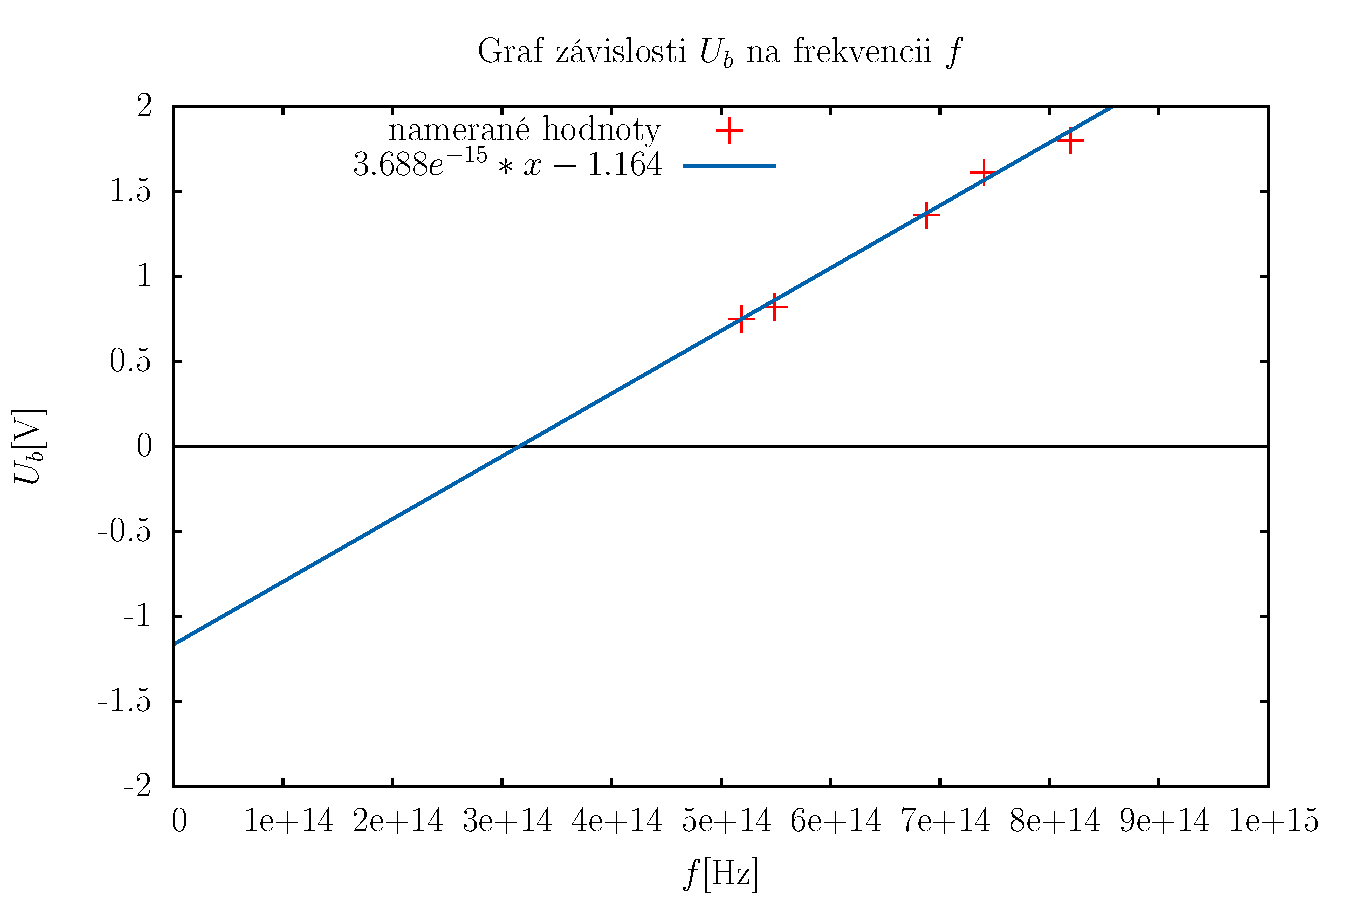
\includegraphics[width=16cm,clip=true]{ify24.pdf}
\end{figure}

\end{document}